% Assign classrooms
Let the set $S$ contain as elements number of students in each course $i$ (denote $s_i$) and set $C$ contain as elements number of chairs in each classroom $j$ (denote $c_j$). We now sort both the sets $S$ and $C$ in ascending order. Since we are trying to minimize the ``disparity" measure ($|s - c|$) over all the assignments, once these sorted numbers are put in a number line the optimal assignment looks like follows: \\



% Define style for nodes
\tikzstyle{every node}=[circle, draw, fill=black!50,
                        inner sep=0pt, minimum width=4pt]
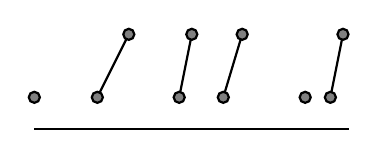
\begin{tikzpicture}[thick,scale=0.8]
	\draw (0,0) node {};
  	\draw (1,0) node {} --  (1.5,1) node {};
  	\draw (2.3,0) node {} --  (2.5,1) node {};
  	\draw (3,0) node {} --  (3.3,1) node {};
  	\draw (4.3,0) node {};
  	\draw (4.7,0) node {} --  (4.9,1) node {};
  	\draw (0, -0.5) -- (5, -0.5);

    
\end{tikzpicture}\quad



We can observe that under optimal assignment the lines assigning courses to classrooms do not cross each other, else it would not be an optimal assignment. In other words, for course $i$ and $j$ with $s_i < s_j$, course $i$ is never assigned a classroom bigger than the one assigned to course $j$. This observation allows us to define subproblems to the original problem in an easy way.

We define $OPT(n', m')$ as the optimal assignment (one that minimizes the cost function) for a sub-problem containing $n'$ courses and $m'$ classrooms where $m' \geq n'$.



Since all courses need to be assigned a classroom, when the arrays are sorted course $n'$ can only be assigned one of the classes with indices in the interval $[n', m']$.

Now the recurrence relation for the subproblem can be formulated as :

\begin{center}
	$OPT(n', m') = \min\limits_{n'\leq k \leq m'} (OPT(n'-1, k-1) + |s_{n'} - c_{k}|)$
\end{center}

So we need to maintain an array of size $mn$ and computing each matrix entry requires $O(m)$ computations, hence finding the optimal solution to the original problem requires $O(nm^2)$ computations.

Now lets see if we can do better.

From the observation that under optimal assignment the lines assigning courses to classrooms do not cross each other (for sorted sequences $S$ and $C$) we can formulate this problem as a sequence alignment problem. We modify the edit distances as follows:

\begin{itemize}
\item cost of mismatch between number of students $s_i$ and number of chairs $c_j$ (corresponding to characters in the sequence) is the absolute value of their difference, i.e $| c_i - s_j |$
\item since $m \geq n$, i.e. number of classrooms has to be larger than number of courses, we disallow deletion of classrooms. Hence cost of deletion of classrooms is set to infinity while cost of insertion is set to 0.   
\end{itemize}

So the total cost of transforming sorted sequence $S$ to $C$ is just the sum of cost due to mismatches, which is what we are trying to minimize. Due to the fact that this is just a sequence alignment problem the complexity is $O(mn)$

